% Using my super cool template

\documentclass[13pt,oneside]{tufte-book}

% ams
\usepackage{amssymb,amsmath}

\usepackage{ifxetex,ifluatex}
\usepackage{fixltx2e} % provides \textsubscript
\ifnum 0\ifxetex 1\fi\ifluatex 1\fi=0 % if pdftex
  \usepackage[T1]{fontenc}
  \usepackage[utf8]{inputenc}
\else % if luatex or xelatex
  \makeatletter
  \@ifpackageloaded{fontspec}{}{\usepackage{fontspec}}
  \makeatother
  \defaultfontfeatures{Ligatures=TeX,Scale=MatchLowercase}
  \makeatletter
  \@ifpackageloaded{soul}{
     \renewcommand\allcapsspacing[1]{{\addfontfeature{LetterSpace=15}#1}}
     \renewcommand\smallcapsspacing[1]{{\addfontfeature{LetterSpace=10}#1}}
   }{}
  \makeatother

\fi

% graphix
\usepackage{graphicx}
\setkeys{Gin}{width=\linewidth,totalheight=\textheight,keepaspectratio}

% booktabs
\usepackage{booktabs}

% url
\usepackage{url}

% hyperref
\usepackage{hyperref}

% units.
\usepackage{units}


\setcounter{secnumdepth}{2}

% citations

% pandoc syntax highlighting
\usepackage{color}
\usepackage{fancyvrb}
\newcommand{\VerbBar}{|}
\newcommand{\VERB}{\Verb[commandchars=\\\{\}]}
\DefineVerbatimEnvironment{Highlighting}{Verbatim}{commandchars=\\\{\}}
% Add ',fontsize=\small' for more characters per line
\newenvironment{Shaded}{}{}
\newcommand{\KeywordTok}[1]{\textcolor[rgb]{0.00,0.44,0.13}{\textbf{#1}}}
\newcommand{\DataTypeTok}[1]{\textcolor[rgb]{0.56,0.13,0.00}{#1}}
\newcommand{\DecValTok}[1]{\textcolor[rgb]{0.25,0.63,0.44}{#1}}
\newcommand{\BaseNTok}[1]{\textcolor[rgb]{0.25,0.63,0.44}{#1}}
\newcommand{\FloatTok}[1]{\textcolor[rgb]{0.25,0.63,0.44}{#1}}
\newcommand{\ConstantTok}[1]{\textcolor[rgb]{0.53,0.00,0.00}{#1}}
\newcommand{\CharTok}[1]{\textcolor[rgb]{0.25,0.44,0.63}{#1}}
\newcommand{\SpecialCharTok}[1]{\textcolor[rgb]{0.25,0.44,0.63}{#1}}
\newcommand{\StringTok}[1]{\textcolor[rgb]{0.25,0.44,0.63}{#1}}
\newcommand{\VerbatimStringTok}[1]{\textcolor[rgb]{0.25,0.44,0.63}{#1}}
\newcommand{\SpecialStringTok}[1]{\textcolor[rgb]{0.73,0.40,0.53}{#1}}
\newcommand{\ImportTok}[1]{#1}
\newcommand{\CommentTok}[1]{\textcolor[rgb]{0.38,0.63,0.69}{\textit{#1}}}
\newcommand{\DocumentationTok}[1]{\textcolor[rgb]{0.73,0.13,0.13}{\textit{#1}}}
\newcommand{\AnnotationTok}[1]{\textcolor[rgb]{0.38,0.63,0.69}{\textbf{\textit{#1}}}}
\newcommand{\CommentVarTok}[1]{\textcolor[rgb]{0.38,0.63,0.69}{\textbf{\textit{#1}}}}
\newcommand{\OtherTok}[1]{\textcolor[rgb]{0.00,0.44,0.13}{#1}}
\newcommand{\FunctionTok}[1]{\textcolor[rgb]{0.02,0.16,0.49}{#1}}
\newcommand{\VariableTok}[1]{\textcolor[rgb]{0.10,0.09,0.49}{#1}}
\newcommand{\ControlFlowTok}[1]{\textcolor[rgb]{0.00,0.44,0.13}{\textbf{#1}}}
\newcommand{\OperatorTok}[1]{\textcolor[rgb]{0.40,0.40,0.40}{#1}}
\newcommand{\BuiltInTok}[1]{#1}
\newcommand{\ExtensionTok}[1]{#1}
\newcommand{\PreprocessorTok}[1]{\textcolor[rgb]{0.74,0.48,0.00}{#1}}
\newcommand{\AttributeTok}[1]{\textcolor[rgb]{0.49,0.56,0.16}{#1}}
\newcommand{\RegionMarkerTok}[1]{#1}
\newcommand{\InformationTok}[1]{\textcolor[rgb]{0.38,0.63,0.69}{\textbf{\textit{#1}}}}
\newcommand{\WarningTok}[1]{\textcolor[rgb]{0.38,0.63,0.69}{\textbf{\textit{#1}}}}
\newcommand{\AlertTok}[1]{\textcolor[rgb]{1.00,0.00,0.00}{\textbf{#1}}}
\newcommand{\ErrorTok}[1]{\textcolor[rgb]{1.00,0.00,0.00}{\textbf{#1}}}
\newcommand{\NormalTok}[1]{#1}

% longtable
\usepackage{longtable,booktabs}

% multiplecol
\usepackage{multicol}

% strikeout
\usepackage[normalem]{ulem}

% morefloats
\usepackage{morefloats}


% tightlist macro required by pandoc >= 1.14
\providecommand{\tightlist}{%
  \setlength{\itemsep}{0pt}\setlength{\parskip}{0pt}}

% title / author / date
\title{Information Theory}
\author{Ashwin Reddy}
\date{}

% header-includes
\usepackage{indent first} \usepackage{tikz-cd} \usepackage{algorithm2e}
\usepackage{mdframed} \usepackage{cancel}
\hypersetup{colorlinks=true, urlcolor=blue} \newcommand{\RR}{\mathbb{R}}
\usepackage{qtree} \usepackage{commath} \usepackage{mathrsfs}
% end of header-includes

\usepackage{amsthm}
\newtheorem{theorem}{Theorem}[chapter]
\newtheorem{lemma}{Lemma}[chapter]
\newtheorem{corollary}{Corollary}[chapter]
\newtheorem{proposition}{Proposition}[chapter]
\newtheorem{conjecture}{Conjecture}[chapter]
\theoremstyle{definition}
\newtheorem{definition}{Definition}[chapter]
\theoremstyle{definition}
\newtheorem{example}{Example}[chapter]
\theoremstyle{definition}
\newtheorem{exercise}{Exercise}[chapter]
\theoremstyle{remark}
\newtheorem*{remark}{Remark}
\newtheorem*{solution}{Solution}
\let\BeginKnitrBlock\begin \let\EndKnitrBlock\end
\begin{document}

{
\surroundwithmdframed{theorem}
\surroundwithmdframed{example}
\surroundwithmdframed{exercise}
}

\maketitle


% include befores
% end of include befores

{
\setcounter{tocdepth}{1}
\tableofcontents
}

\listoftables
\listoffigures

\chapter{Introduction}\label{introduction}

Often, lecture notes like these jump into the material without
establishing the basics. This chapter will cover why this book exists
and how to use it.

\section{Philosophy}\label{philosophy}

Two other sets of notes for this course are available at
\url{https://github.com/mananshah99/infotheory} and
\url{http://tiny.cc/infotheory1} . My goal in preparing \emph{this} book
was simply to ensure that I understand the concepts. As a result, I've
spared no expense in filling these notes with as much content as needed
to develop the theory from first principles.

It's also worth noting that the stylistic choices I've made here are
very opinionated. The margins are very wide and are filled with
important asides and footnotes. This format is a result of choosing to
use Edward Tufte's style. Additionally, I've tried to stick to the
typical definition-theorem-proof style with explanatory prose in
between.

Making this book has been a labor of love, requiring more time than I
care to admit. Hopefully, it is a useful resource for you.

\section{Prerequisites}\label{prerequisites}

This book really only assumes a working proficiency with single-variable
calculus (which even then is mostly for intuition) and some familiarity
with multivariable calculus. Important concepts of probability are
developed from scratch, however. Intuition is heavily emphasized.

\section{Why study Information
Theory?}\label{why-study-information-theory}

Information Theory is a mathematical framework for thinking about what
it means to have efficient communication. Examples of information
include:

\begin{itemize}
\tightlist
\item
  Email
\item
  Telegraph
\item
  Images
\item
  Speech
\item
  Video
\end{itemize}

Much of today's digital world revolves around transmitting information:
we zip files, email them across the internet, download MP3s, etc. The
ideas of information theory give us a rigorous way of characterizing
streams of information. The cornerstone of our model will start with the
following pipeline of sorts

\begin{figure}
\centering
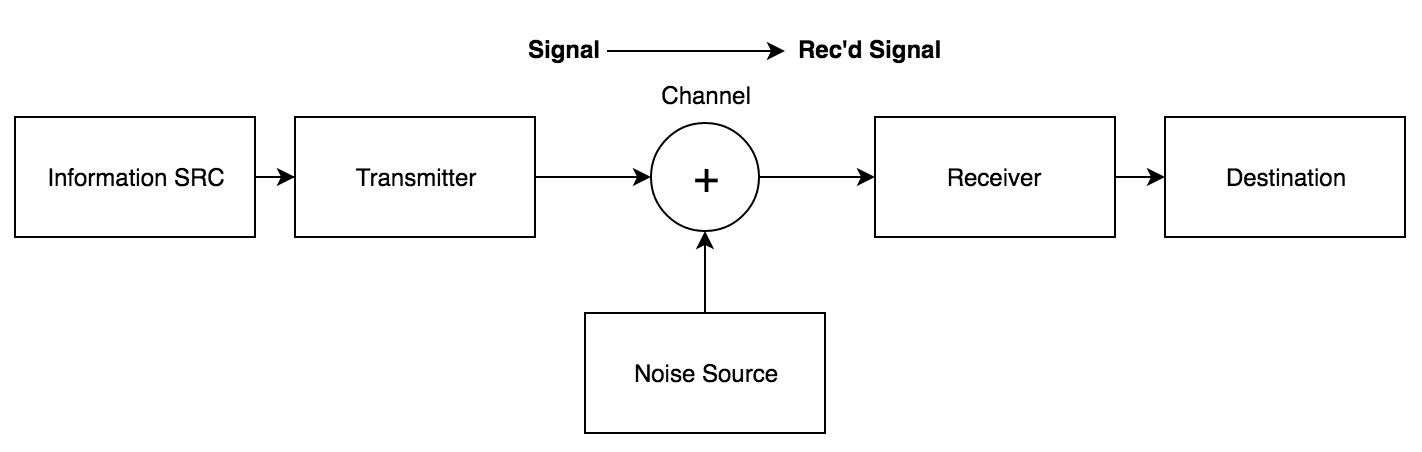
\includegraphics{pipeline.png}
\caption{}
\end{figure}

This model gives us a general way of abstracting the transmission of
information. On the left we have a source of information (where a signal
originates) that is sent to a transmitter. A channel then allows that
signal to flow to a receiver, although noise may be added at this stage.
Finally, the receiver sends the signal to the destination. Right now,
this model may not be very elucidating. However, we will see that it
gives us a structure within which we can consider various mathematical
characterizations of information. However, before we can begin to
consider information in depth, we must first start our foundation with a
solid understanding of probability as that is the underlying theory
below Information Theory.

\part{Theory}\label{part-theory}

\chapter{Stochastic Variables}\label{stochastic-variables}

\BeginKnitrBlock{definition}[Stochastic Variable]
\protect\hypertarget{def:unnamed-chunk-2}{}{\label{def:unnamed-chunk-2}
\iffalse (Stochastic Variable) \fi{} } A \textbf{stochastic variable} is
a real-valued function of an outcome of an experiment.
\EndKnitrBlock{definition}

\BeginKnitrBlock{remark}
\iffalse{} {Remark. } \fi{} Stochastic variables are also called random
variables, but this term seems to imply all possibilities are equally
likely or cannot be determined. The word stochastic generally means
something like ``depending upon probabilities.''
\EndKnitrBlock{remark}

\BeginKnitrBlock{example}
\protect\hypertarget{exm:unnamed-chunk-4}{}{\label{exm:unnamed-chunk-4} }
Toss a coin 7 times. The number of heads in the sequence could be a
stochastic variable.
\EndKnitrBlock{example}

\BeginKnitrBlock{remark}
\iffalse{} {Remark. } \fi{} The 7-long sequence itself is not a
stochastic variable, since it is not a real value. We should always have
a clear way of assigning a real number to the outcome.
\EndKnitrBlock{remark}

\BeginKnitrBlock{example}
\protect\hypertarget{exm:unnamed-chunk-6}{}{\label{exm:unnamed-chunk-6} }
Sum two rolls of a die. This value could be a stochastic variable. The
number of 5's rolled could also be a stochastic variable.
\EndKnitrBlock{example}

A stochastic variable can either be discrete, taking on values from a
countable set or continuous, taking on values on an interval from the
real number line \(\mathbb{R}\).

\section{Probability Measure}\label{probability-measure}

\BeginKnitrBlock{definition}[Sample Space]
\protect\hypertarget{def:unnamed-chunk-7}{}{\label{def:unnamed-chunk-7}
\iffalse (Sample Space) \fi{} } The \textbf{sample space} is the set of
all possible outcomes for an experiment.
\EndKnitrBlock{definition}

\begin{marginfigure}
The sample space is typically represented with \(\Omega\).
\end{marginfigure}

\BeginKnitrBlock{definition}[Event]
\protect\hypertarget{def:unnamed-chunk-9}{}{\label{def:unnamed-chunk-9}
\iffalse (Event) \fi{} } An \textbf{event} is a subset of the sample
space \(\Omega\).
\EndKnitrBlock{definition}

\BeginKnitrBlock{remark}
\iffalse{} {Remark. } \fi{} Any event belongs to the power set of
\(\Omega\).\footnote{The Wikipedia article on
  \href{https://en.wikipedia.org/wiki/Event_(probability_theory)\#A_simple_example}{events}
  has good examples.} Thus, events range from the empty set to a
singleton set (i.e.~a set with size unity) to \(\Omega\) itself and
anything in between.
\EndKnitrBlock{remark}

\begin{marginfigure}
\begin{tikzcd}
 & X \arrow{dr}{\text{can take on values from}} \\
\Pr \arrow{ur}{\text{function of}} \arrow{rr}{\text{of specific value}} && x
\end{tikzcd}
\end{marginfigure}

\BeginKnitrBlock{definition}[Probability Measure]
\protect\hypertarget{def:unnamed-chunk-12}{}{\label{def:unnamed-chunk-12}
\iffalse (Probability Measure) \fi{} } The \textbf{probability measure}
\(\Pr\) is a real-valued function that assigns events probabilities
obeying the \textbf{Kolmogorov axioms}.
\EndKnitrBlock{definition}

\BeginKnitrBlock{remark}
\iffalse{} {Remark. } \fi{} Our notions of probability are fairly
intuitive, so a careful treatment of the Kolmogorov axioms is not
needed. They are available in the \protect\hyperlink{kmaxm}{appendix},
however.
\EndKnitrBlock{remark}

If each element of an event \(A\) is equally likely, then

\[
\Pr(A) = \frac{|A|}{|\Omega|}
\]

\begin{marginfigure}
\textbf{Notation}. In general, if \(X\) is a stochastic variable, the
probability mass function can be written in two equivalent ways:

\begin{equation}
p_X(x) = \Pr(X=x)
\label{eq:prob-notation}
\end{equation}
\end{marginfigure}

\section{Bayes' Theorem}\label{bayes-theorem}

Events \(A\) and \(B\) are said to be independent if the occurence of
one does not affect the probabilities of the other. When events \(A\)
and \(B\) are not independent, knowing what \(A\) is gives us
information about what \(B\) might be (and vice versa). The notation
\(\Pr(A|B)\) denotes the probability of \(A\) given that or conditioned
upon \(B\) occuring. Consider that for \(A\) and \(B\) to happen that
\(B\) must first happen and \(A\) must happen under those circumstances.

\begin{equation}
\Pr(A \cap B)  = \Pr(B) \cdot \Pr\left(A | B\right) 
\label{eq:conditional-prob}
\end{equation}

From this definition, Thomas Bayes determined how to compute the support
\(B\) provides for \(A\) given \emph{priors} and \emph{posteriors}.

\BeginKnitrBlock{theorem}[Bayes' Theorem]
\protect\hypertarget{thm:unnamed-chunk-15}{}{\label{thm:unnamed-chunk-15}
\iffalse (Bayes' Theorem) \fi{} } \[
\Pr( A|B) = \frac{\Pr(B|A)\Pr(A)}{\Pr(B)}
\]
\EndKnitrBlock{theorem}

\BeginKnitrBlock{proof}
\iffalse{} {Proof. } \fi{} Equation \eqref{eq:conditional-prob} is
symmetric since \(A\) and \(B\) is the same as \(B\) and \(A\). Thus,
\(\Pr(A|B)\Pr(B) = \Pr(B|A)\Pr(B)\).
\EndKnitrBlock{proof}

\section{Probability Mass Functions}\label{probability-mass-functions}

A \textbf{probability mass function} (pmf) characterizes a discrete
stochastic variable by returning the probability measure of some \(x\)
in \(\Omega\) occuring.

\BeginKnitrBlock{example}
\protect\hypertarget{exm:unnamed-chunk-17}{}{\label{exm:unnamed-chunk-17} }
Consider 2 tosses of a fair coin. What is the probability mass function
(pmf) of the number of heads given this experiment?
\EndKnitrBlock{example}

\BeginKnitrBlock{solution}
\iffalse{} {Solution. } \fi{} It is useful to construct a table of all
the possibilities.

\begin{longtable}[]{@{}lll@{}}
\toprule
& Heads & Tails\tabularnewline
\midrule
\endhead
Heads & 2 & 1\tabularnewline
Tails & 1 & 0\tabularnewline
\bottomrule
\end{longtable}

From the table, we can conclude that

\[
\Pr(X=x) = \begin{cases}
1/4 & x = 0 \\
1/2 & x = 1 \\
1/4 & x = 2 \\
0 & \text{otherwise}
\end{cases}
\]
\EndKnitrBlock{solution}

\BeginKnitrBlock{example}
\protect\hypertarget{exm:unnamed-chunk-19}{}{\label{exm:unnamed-chunk-19} }
Consider a 4-sided die rolled twice. What is the probability mass
function for the maximum value of 2 rolls?
\EndKnitrBlock{example}

\BeginKnitrBlock{solution}
\iffalse{} {Solution. } \fi{}

As before, let us think about the various possibilities. There are
\(4 \times 4 = 16\) total possibilities, and the maximum value can take
on values 1, 2, 3, and 4. To take on a value of 1, both rolls must have
been a 1; the probability of this happening is 1/16. To take on a value
of 2, one of the rolls must have been a 2 and the other one must have
been a 1 or a 2. The possibilites are enumerated as (2,1), (2,2), (1,2).
Thus, its chance is 3/16. For a max value of 3, the possibilities are
(3,1), (3,2), (3,3), (1,3), (2,3). Thus,

\[
p_X(x) = \begin{cases}
1/16 & x = 1 \\
3/16 & x = 2 \\
5/16 & x = 3 \\
7/16 & x = 4 \\
0 & \text{otherwise}
\end{cases}
\]
\EndKnitrBlock{solution}

There are a few common discrete stochastic variables that are worth
discussing separately. The chapter on
\protect\hyperlink{discrete-stochastic-variables}{Discrete Stochastic
Variables} covers 4 important ones. The following sections will assume
familiarity with these variables.

\section{Expectation and Variance}\label{expectation-and-variance}

As is often the case in mathematics, we like to define general operators
on objects to understand their properties. Firstly, note that we can use
functions of stochastic variables to build other stochastic variables.

\BeginKnitrBlock{example}[Simple Functions of a Stochastic Variable]
\protect\hypertarget{exm:unnamed-chunk-21}{}{\label{exm:unnamed-chunk-21}
\iffalse (Simple Functions of a Stochastic Variable) \fi{} }Consider the
following pmf

\[
p_X(x) = \begin{cases}
1/9 & x \in \{ -4, -3, -2, -1, 0, 1, 2, 3, 4\} \\
0 & \text{otherwise}
\end{cases}
\] Here are two functions of \(X\) and their probability mass functions:

\begin{enumerate}
\def\labelenumi{\alph{enumi})}
\tightlist
\item
  \(Y=|X| \implies p_Y(y)=\begin{cases}2/9 & y \in \{1,2,3,4\} \\ 1/9 & y=0 \end{cases}\)
\item
  \(Z=X^2 \implies p_Z(z)=\begin{cases}2/9 & z \in \{1,4,9,16\} \\ 1/9 & z=0 \end{cases}\)
\end{enumerate}
\EndKnitrBlock{example}

A special class of functions, known as moments, include two operators,
\textbf{expectation} and \textbf{variance}.

\BeginKnitrBlock{definition}[Expectation]
\protect\hypertarget{def:unnamed-chunk-22}{}{\label{def:unnamed-chunk-22}
\iffalse (Expectation) \fi{} } The expectation of a function \(g\) of a
stochastic variable \(X\) is

\[
\mathbb{E}[g(X)] \equiv \sum_{x \in \Omega} g(x) \cdot \Pr(X=x)
\]
\EndKnitrBlock{definition}

Expectation returns the mean of the function \(g\), that is, what we
expect the average value of \(g(X)\) to be if we run the experiment an
infinite number of times.

\BeginKnitrBlock{exercise}[Expected Value of a Die]
\protect\hypertarget{exr:unnamed-chunk-23}{}{\label{exr:unnamed-chunk-23}
\iffalse (Expected Value of a Die) \fi{} } Find \(\mathbb{E}[X]\) where
\(X\) is the value of a roll of a die.
\EndKnitrBlock{exercise}

\BeginKnitrBlock{solution}
\iffalse{} {Solution. } \fi{} Each value has a \(1/6\) chance of
appearing. Therefore,

\[
\mathbb{E}[X] = \sum_{i=1}^6 \frac{1}{6}i = \frac{21}{6} = 3.5
\]

We include a numerical solution showing convergence:
\EndKnitrBlock{solution}

\begin{Shaded}
\begin{Highlighting}[]
\NormalTok{N  }\OperatorTok{=} \DecValTok{1000}\OperatorTok{;}\NormalTok{ plt.plot(np.cumsum(np.random.randint(}\DecValTok{1}\NormalTok{, }\DecValTok{7}\NormalTok{, size}\OperatorTok{=}\NormalTok{N)) }\OperatorTok{/}\NormalTok{ np.arange(}\DecValTok{1}\NormalTok{, N }\OperatorTok{+} \DecValTok{1}\NormalTok{))}
\end{Highlighting}
\end{Shaded}

\includegraphics{info-theory_files/figure-latex/unnamed-chunk-26-1}

\BeginKnitrBlock{theorem}[Linearity of Expectation]
\protect\hypertarget{thm:unnamed-chunk-27}{}{\label{thm:unnamed-chunk-27}
\iffalse (Linearity of Expectation) \fi{} }\[
\mathbb{E}\left[aX+bY\right] = a\mathbb{E}[X]+b\mathbb{E}[Y]
\]
\EndKnitrBlock{theorem}

\begin{marginfigure}
The \(n\)th moment about \(x_0\) is defined as
\(\mathbb{E}[(x-x_0)^n]\).
\end{marginfigure}

\BeginKnitrBlock{definition}[Variance]
\protect\hypertarget{def:unnamed-chunk-29}{}{\label{def:unnamed-chunk-29}
\iffalse (Variance) \fi{} } The variance is the 2nd moment about the
mean.

\begin{equation}
\mathrm{Var}[X] \equiv \mathbb{E}[(X-\mathbb{E}[X])^2]
\label{eq:variance-def}
\end{equation}
\EndKnitrBlock{definition}

Unfortunately, the definition given above in Equation
\eqref{eq:variance-def} tends to be difficult to compute by hand. A little
algebra results in a computationally simpler alternative.

\BeginKnitrBlock{lemma}[Determinism of Expectation of Expectation]
\protect\hypertarget{lem:unnamed-chunk-30}{}{\label{lem:unnamed-chunk-30}
\iffalse (Determinism of Expectation of Expectation) \fi{} }\[
\mathbb{E}\Big[\mathbb{E}[X]\Big] = \mathbb{E}[X]
\]
\EndKnitrBlock{lemma}

\BeginKnitrBlock{theorem}[Computationally Simpler Alternative for Variance]
\protect\hypertarget{thm:unnamed-chunk-31}{}{\label{thm:unnamed-chunk-31}
\iffalse (Computationally Simpler Alternative for Variance) \fi{} }

\begin{equation}
\mathrm{Var}[X] = \mathbb{E}[X^2] - \mathbb{E}\left[X\right]^2
\label{eq:variance-comp}
\end{equation}
\EndKnitrBlock{theorem}

\BeginKnitrBlock{proof}
\iffalse{} {Proof. } \fi{}

\begin{align*}
\mathrm{Var}[X] &= \mathbb{E}\Big[X^2 + \mathbb{E}[X]^2 - 2X\mathbb{E}[X]\Big] \\
&= \mathbb{E}[X^2] + \mathbb{E}[X]^2 - 2\mathbb{E}[X]\mathbb{E}[X] \\
&= \mathbb{E}[X^2] - \mathbb{E}[X]^2.
\end{align*}
\EndKnitrBlock{proof}

\begin{marginfigure}
As an aside, the indicator function \(\mathbb{1}_A\) indicates whether
certain events are in \(A\) or not.

\[
\mathbb{1}_A(\omega) = \begin{cases} 1 & \omega \in A \\ 0 & \omega \not\in A \end{cases}
\]

As a result,

\[\mathbb{E}[\mathbb{1}_A(\omega)] = \Pr(A)\]
\[\mathrm{Var}[\mathbb{1}_A(\omega)] = P(A)(1-P(A))\]
\end{marginfigure}

\BeginKnitrBlock{lemma}
\protect\hypertarget{lem:unnamed-chunk-34}{}{\label{lem:unnamed-chunk-34} }
If \(X\) and \(Y\) are independent,

\[
\operatorname{Var}[X+Y] = \operatorname{Var}[X] + \operatorname{Var}[Y]
\]
\EndKnitrBlock{lemma}

\BeginKnitrBlock{proof}
\iffalse{} {Proof. } \fi{}

\begin{align*}
\operatorname{Var}[X+Y] &= \mathbb{E}[(X+Y)^2] - \mathbb{E}[X+Y]^2 \\
&= \mathbb{E}[X^2 + 2XY + Y^2] - \mathbb{E}[X+Y]^2 \\
&= \mathbb{E}[X^2] + 2\mathbb{E}[XY] + \mathbb{E}[Y^2] - (\mathbb{E}[X+Y])^2 \\
&= \mathbb{E}[X^2] + 2\mathbb{E}[X]\mathbb{E}[Y] + \mathbb{E}[Y^2] - \left( \mathbb{E}[X]^2 + 2\mathbb{E}[X]\mathbb{E}[Y] + \mathbb{E}[Y]^2 \right) \\
&= \mathbb{E}[X^2] + 2\mathbb{E}[X]\mathbb{E}[Y] + \mathbb{E}[Y^2] - \mathbb{E}[X]^2 - 2\mathbb{E}[X]\mathbb{E}[Y] - \mathbb{E}[Y]^2 \\
&= \mathbb{E}[X^2] - \mathbb{E}[X]^2 + \mathbb{E}[Y^2] - \mathbb{E}[Y]^2 \\
&= \operatorname{Var}[X] + \operatorname{Var}[Y]
\end{align*}
\EndKnitrBlock{proof}

\begin{longtable}[]{@{}lll@{}}
\caption{Expectation and Variance of Common
Distributions}\tabularnewline
\toprule
Distribution & Expectation & Variance\tabularnewline
\midrule
\endfirsthead
\toprule
Distribution & Expectation & Variance\tabularnewline
\midrule
\endhead
Binomial & \(np\) & \(np(1-p)\)\tabularnewline
Geometric & \(1/p\) & \((1-p)/p^2\)\tabularnewline
Poisson & \(\lambda\) & \(\lambda\)\tabularnewline
\bottomrule
\end{longtable}

\section{Probability Density
Functions}\label{probability-density-functions}

Now we turn to stochastic variables that return values on an interval of
the real number line. We can use our knowledge of discrete stochastic
variables to find analagous versions for continuous stochastic
variables. Instead of a probability mass function, we call the function
for a continuous stochastic variables \textbf{probability density
function} (pdf).

\begin{marginfigure}
\textbf{Notation}. Probability density functions are typically denoted
with lowercase English letters, most commonly \(f\).
\end{marginfigure}

The requirement that the total probability must add up to unity is still
in place:

\[
\int_{\mathbb{R}} f_X(x)\,\mathrm{d}x=1
\]

However, asking whether \(X=x\) is no longer a well-formed question,
since \(X\) has a continuum. The probability that \(X\) takes on the
exact value \(x\) is nil. Therefore, probabilities of a continuous
stochastic variable may only be queried in the following form.

\[
\Pr(a\leq X \leq b) = \int\limits_{a}^{b}f_X(x)\,\mathrm{d}x
\]

By extension, the expectation of a pdf can be computed as

\[
\mathbb{E}[X] = \int_{\mathbb{R}}xf_X(x)\,\mathrm{d}x
\]

The chapter on
\protect\hyperlink{continuous-stochastic-variables}{Continuous
Stochastic Variables} discusses 3 important stochastic variables:
uniform, exponential, and Gaussian. These variables will come up later,
but for the sake of cleanliness, the proofs and computations have been
moved into the appendix.

\chapter{Entropy}\label{entropy}

Why did we spend the time reviewing probability for information? The
answer lies in Proposition \ref{prp:stochasticity-of-info} below:

\BeginKnitrBlock{proposition}[Stochasticity of Information]
\protect\hypertarget{prp:stochasticity-of-info}{}{\label{prp:stochasticity-of-info}
\iffalse (Stochasticity of Information) \fi{} } Information can be
modelled as samples from a stochastic source.
\EndKnitrBlock{proposition}

Consider the fact that many emails you send will have a typical
structure: a greeting, a body of text, a conclusion. Or that the changes
in the frames of a video tend to be rather small. Intuitively, we have a
sense that the repetitive elements of data are not information-dense,
and therefore, when we transmit this information, we should really only
focus on what is novel about each message.

Shannon's original example was to show that text can modelled
probabilistically in this way. Let's imagine that we want to generate
some text that looks like English. We can first start by creating a
sample space \(\Omega\) that includes letters and spaces. Then, we
sample randomly. This is callled a zero-order approximation. Next, we
can refine the approximation by making characters more or less frequent.
Adapting the probability based on the frequency with which that
character appears in a corpus (e.g.~make \emph{e} show up about 12\% of
the time) is called a first-order approximation. An even more refined
approach would consider digram (2-character sequences) and their
frequencies.

\section{Surprisal}\label{surprisal}

Now that you're convinced that information can be modelled
stochastically, we can consider what information means.

\BeginKnitrBlock{example}[The Q-U Question]
\protect\hypertarget{exm:unnamed-chunk-37}{}{\label{exm:unnamed-chunk-37}
\iffalse (The Q-U Question) \fi{} } Consider a game where you predict
the next letter of a piece of English text given all the previous
letters. You are given the phrase \texttt{elephants\ are\ q}. You know
that the letter \texttt{q} is nearly always followed by a \texttt{u}.
You would then predict that the next letter is a \texttt{u}, and you
would be confident in your guess. If, by some odd reason, that next
letter is not a \texttt{u}, you would be ``surprised''.
\EndKnitrBlock{example}

What we've captured in this example is a working conception of
information.

\BeginKnitrBlock{definition}[Information]
\protect\hypertarget{def:unnamed-chunk-38}{}{\label{def:unnamed-chunk-38}
\iffalse (Information) \fi{} } New information (which is really the only
kind of information we care about) \textbf{is} the ``surprisal'' of an
information source. The more surprised you are, the more information you
gain, since you didn't expect to see that result.
\EndKnitrBlock{definition}

\begin{marginfigure}
Shannon's formula for entropy actually has a similarity to thermodynamic
entropy:

\[
S = - k_B \sum p_i \ln p_i
\]
\end{marginfigure}

We now need a way of quantifying surprisal/information. The core of our
theory is that surprisal should be inversely correlated with the
probability of occurence. So naturally, we gravitate towards picking
something like \(1/p\) as our information function. Consider the limit
cases, however, of literally using \(1/p\). When \(p=0\), we have
infinite surprisal, and when \(p=1\), we have 1 unit of surprisal. If
something is guaranteed to happen, 1 unit is an odd baseline to use. As
a result, we pick \(\log(1/p)\), which is more attractive for a few
reasons.

\begin{enumerate}
\def\labelenumi{\arabic{enumi}.}
\tightlist
\item
  Continuity
\item
  Monotonically decreasing in \(p\)
\item
  Never negative
\item
  With \(p=1\), information becomes 0
\item
  Information due to independent events is additive
\end{enumerate}

\begin{marginfigure}
Typically, we will pick a base of \(2\) although any other sensible base
works. We will usually omit the subscript/base unless it needs to be
made explicit.
\end{marginfigure}

To each event, we now attach a surprisal value. To characterize a
stochastic variable as a whole, we now define entropy.

\BeginKnitrBlock{definition}[Entropy]
\protect\hypertarget{def:unnamed-chunk-41}{}{\label{def:unnamed-chunk-41}
\iffalse (Entropy) \fi{} } The entropy \(H\) of a stochastic variable
\(X\) is the expectation of surprisal of \(X\).

\begin{align*}
H(X) &\equiv \mathbb{E}\left[\log \frac{1}{\Pr(X=x)}\right]\\
&= \sum_i p_i \log(1/p_i) \\
&= -\sum_i p_i \log p_i
\end{align*}
\EndKnitrBlock{definition}

\BeginKnitrBlock{lemma}[Entropy is Nonnegative]
\protect\hypertarget{lem:nonnegative-entropy}{}{\label{lem:nonnegative-entropy}
\iffalse (Entropy is Nonnegative) \fi{} }\[
\forall X, H(X) \geq 0
\]
\EndKnitrBlock{lemma}

\BeginKnitrBlock{proof}
\iffalse{} {Proof. } \fi{}

\begin{gather*}
H(X) \geq 0 \\
-\sum_{x \in \Omega} \Pr(X=x)\log\Pr(X=x) \geq 0 \\
\sum_{x \in \Omega} \Pr(X=x)\log\Pr(X=x) \leq 0 \\
\end{gather*}

Note that
\[\forall x \in \Omega, 0\leq \Pr(X=x) \leq 1 \implies \forall x \in \Omega, \log\Pr(X=x) \leq 0.\]
Since a weighted sum of negative numbers with nonegative numbers can
never be positive, entropy can never be negative.
\EndKnitrBlock{proof}

\BeginKnitrBlock{exercise}[Entropy of Bernoulli Distribution]
\protect\hypertarget{exr:bern-entropy}{}{\label{exr:bern-entropy}
\iffalse (Entropy of Bernoulli Distribution) \fi{} } Find the entropy of
a general Bernoulli distribution and plot the entropy against the
probability of heads.
\EndKnitrBlock{exercise}

\BeginKnitrBlock{solution}
\iffalse{} {Solution. } \fi{}

\[
H(X) = p \log \frac{1}{p} + (1-p)\log \frac{1}{1-p}
\]

Plotting for every possible value for \(p\), we yield a nice graph:
\EndKnitrBlock{solution}

\begin{figure}
\includegraphics{info-theory_files/figure-latex/unnamed-chunk-44-1} \caption[Bernoulli Entropy]{Bernoulli Entropy}\label{fig:unnamed-chunk-44}
\end{figure}

When \(p\) is 0 or 1, we need 0 bits of information, which makes sense
because the result was guaranteed. As we go more towards complete
randomness (which colloquially, we might also call ``entropy'' from a
physics standpoint), we need more bits to represent the possibilites (a
maximum of 1 in this case).

\BeginKnitrBlock{remark}
\iffalse{} {Remark. } \fi{} But what does it mean to have 0.47 bits,
which we might have if \(p(\text{heads})=0.9\)? Imagine that we had a
100-long sequence of coin flips and we transmitted the information. For
the purely random case (i.e.~using a fair coin), we would need 100 bits.
However, for this extremely unfair case, we could get away with 47 bits
without losing any information (on average).
\EndKnitrBlock{remark}

\section{Bit Representations}\label{bit-representations}

While we will be overloading the word bit in different contexts in this
book, it is useful to understand what it represents. As noted before,
bit is an abbreviation of ``binary digit.'' When we talk about a bit in
computer science, we typically mean 0 or 1, low voltage or high voltage,
etc. Here, we take a bit to mean something like the answer to a single
yes or no question with yes and no equally likely. In other words, a
coin toss. That is, one bit captures the information of a Bernoulli
distribution with \(p=0.5\). From there, we can meaningfully interpret
values of entropy as telling us roughly how many of these yes/no
questions or coin flips or sequence of binary digits are needed to
transmit the information on average.

\BeginKnitrBlock{exercise}[Entropy of a Fair Dice Roll]
\protect\hypertarget{exr:fair-dice-roll}{}{\label{exr:fair-dice-roll}
\iffalse (Entropy of a Fair Dice Roll) \fi{} } Find the entropy of a
fair dice roll.
\EndKnitrBlock{exercise}

\BeginKnitrBlock{solution}
\iffalse{} {Solution. } \fi{}

Note that entropy does not care about the actual values of \(X\).
Therefore, the entropy is computed as

\begin{align*}
H(x) &= \sum_x p(x)\log(1/p(x)) \\
&= \sum_{x=1}^6 \frac{1}{6}\log(6) \\
&= 6\cdot\frac{1}{6}\log(6) \\
&= \log 6 \approx 2.585
\end{align*}
\EndKnitrBlock{solution}

\BeginKnitrBlock{exercise}[Double the Possibilities]
\protect\hypertarget{exr:unnamed-chunk-47}{}{\label{exr:unnamed-chunk-47}
\iffalse (Double the Possibilities) \fi{} } Repeat Exercise
\ref{exr:fair-dice-roll} except that there are double the number of
possible values (i.e.~a 12-sided die).
\EndKnitrBlock{exercise}

\BeginKnitrBlock{solution}
\iffalse{} {Solution. } \fi{} Intuitively, we just need to add one more
bit to flip between the first 6 and last 6 values. Mathematically, we
consider \(\log(12)\), which by log properties is
\(\log(2) + \log(6) = 1 + \log(6)\).
\EndKnitrBlock{solution}

\section{Jensen's Inequality}\label{jensens-inequality}

\BeginKnitrBlock{definition}[Convex Function]
\protect\hypertarget{def:unnamed-chunk-49}{}{\label{def:unnamed-chunk-49}
\iffalse (Convex Function) \fi{} } A function \(f(x)\) is
\textbf{convex} on the interval \((a,b)\) if it is concave up on that
interval (i.e.~second derivative is positive).
\EndKnitrBlock{definition}

Alternatively, it obeys the property that for all \((x_1, x_2)\) within
the interval \((a,b)\) and for all \(\lambda\) normalized between 0 and
1,

\[
f(\lambda x_1 + (1-\lambda)x_2) \leq \lambda f(x_1) + (1-\lambda) f(x_2)
\]

\BeginKnitrBlock{theorem}[Jensen's Inequality]
\protect\hypertarget{thm:unnamed-chunk-50}{}{\label{thm:unnamed-chunk-50}
\iffalse (Jensen's Inequality) \fi{} }For a stochastic variable \(X\)
and a convex function \(f\),

\[
\mathbb{E}[f(X)] \geq f(\mathbb{E}[X])
\]
\EndKnitrBlock{theorem}

Intuitively, if we think of expected value as an average, it makes sense
that the average value of a convex function would never exceed the
function's value at its average (i.e.~its midpoint).

\BeginKnitrBlock{theorem}
\protect\hypertarget{thm:max-entropy}{}{\label{thm:max-entropy} }If \(X\)
assumes real values \(\{x_1, \dots, x_n\}\) and
\(0 \leq H(X) \leq \log r\). Then,

\[
\forall\, 1 \leq i \leq n,  p_i = \frac{1}{r} \iff  H(X)=\log r 
\]
\EndKnitrBlock{theorem}

Theorem \ref{thm:max-entropy} tells us that an equiprobable distribution
maximizes entropy. We now see that the intuition from Exercise
\ref{exr:bern-entropy} can be generalized.

\section{Joint \& Conditional Entropy}\label{joint-conditional-entropy}

\BeginKnitrBlock{definition}[Joint Entropy]
\protect\hypertarget{def:unnamed-chunk-51}{}{\label{def:unnamed-chunk-51}
\iffalse (Joint Entropy) \fi{} }\[
H(X,Y) \equiv -\sum_{x}\sum_{y} \Pr(x,y)\log(\Pr(x,y))
\]
\EndKnitrBlock{definition}

\BeginKnitrBlock{definition}[Conditional Entropy]
\protect\hypertarget{def:unnamed-chunk-52}{}{\label{def:unnamed-chunk-52}
\iffalse (Conditional Entropy) \fi{} }\[
H(Y | X) \equiv \sum_x \Pr(X = x) H(Y | X = x)
\]
\EndKnitrBlock{definition}

\BeginKnitrBlock{theorem}
\protect\hypertarget{thm:joint-conditional}{}{\label{thm:joint-conditional}
}

\begin{equation}
H(X,Y) = H(X) + H(Y  | X) = H(Y) + H(X | Y)
\label{eq:joint-conditional}
\end{equation}
\EndKnitrBlock{theorem}

Intuitively, we can think of Equation \eqref{eq:joint-conditional} as
saying that a complete characterization of correlated variables \(X\)
and \(Y\) can be described using as many bits needed to fully describe
\(X\) and then however many additional bits it takes to describe \(Y\)
given \(X\) (and vice versa).

Given that we have different kinds of entropy, it is helpful to write
down one equation that makes the definitions easier to digest:

\begin{equation}
H(\cdot) = \mathbb{E}\left[\log\frac{1}{\Pr(\cdot)}\right]
\label{eq:general-discrete-entropy}
\end{equation}

Equation \eqref{eq:general-discrete-entropy} generates \(H(X)\),
\(H(X,Y)\) and \(H(X|Y)\).

\BeginKnitrBlock{theorem}
\protect\hypertarget{thm:unnamed-chunk-53}{}{\label{thm:unnamed-chunk-53} }
Let \(X\) be a stochastic variable and \(g\) a function of \(X\). Then,

\[
H(g(X)) \leq H(X)
\]
\EndKnitrBlock{theorem}

\BeginKnitrBlock{proof}
\iffalse{} {Proof. } \fi{} Using Theorem \ref{thm:joint-conditional}, we
can expand

\[
H(X, g(X)) = H(X) + H(g(X)|X)
\]

However, \(g(X)\) is completely determined by \(X\). In other words, no
additional bits are needed to describe \(g(X)\) if one has the bits
describing \(X\). Thus, \(H(g(X)|X)=0\), and

\begin{equation}
H(X,g(X)) = H(X).
\label{eq:no-info}
\end{equation}

Additionally, we can use the alternate symmetric expansion

\[
H(X, g(X)) = H(g(X)) + H(X|g(X))
\]

If \(g\) happens to be an injective function, then \(H(X|g(X))=0\) since
knowing \(g(x)\) allows us to trace back the specific \(x\) which
generated it. However, injectivity is not guaranteed. In general, \(g\)
could take different \(x\) inputs and produce the same output with them.
This conflation means that we would require additional bits. Whether
injective or not, we can guarantee that \(H(g(X)) + H(X|g(X))\) will not
be lower than \(H(g(X))\). Or, more to the point,

\begin{equation}
H(X,g(X)) \geq H(g(X)).
\label{eq:at-least-info}
\end{equation}

We now combine Equations \eqref{eq:no-info} and \eqref{eq:at-least-info} to
assert that \(H(g(X)) \leq H(X)\).
\EndKnitrBlock{proof}

Interestingly, we can use conditional entropy to define a
\textbf{metric}.

\BeginKnitrBlock{definition}[Metric]
\protect\hypertarget{def:unnamed-chunk-55}{}{\label{def:unnamed-chunk-55}
\iffalse (Metric) \fi{} } A metric on a set \(X\) is a function
\(d: X \times X \to [0, \infty]\) that defines distance with the
following constraints:

\begin{enumerate}
\def\labelenumi{\arabic{enumi}.}
\tightlist
\item
  \(\forall x, y \in X: d(x,y) \geq 0\)
\item
  \(\forall x, y\in X: d(x,y) = 0 \iff x = y\)
\item
  \(\forall x, y \in X: d(x,y) = d(y,x)\)
\item
  \(\forall x, y, z\in X: d(x,z) \leq d(x,y) + d(y,z)\)
\end{enumerate}
\EndKnitrBlock{definition}

Our goal is to show that \(d(X,Y) = H(X|Y) + H(Y|X)\) works. From Lemma
\ref{lem:nonnegative-entropy}, property (1) should clearly be true. Our
intuition should match up with property (2): the only way to be 0 is if
the number of bits that describes \(X\) completely describes \(Y\).
Property (3) should also be clear by symmetry. Property (4),
intuitively, says that it takes less bits to describe \(X\) and \(Z\)
together than to describe \(X\) and \(Y\) and \(Y\) and \(Z\)
(effectively, all 3).

\section{Differential Entropy}\label{differential-entropy}

We would now like to generalize the concept of entropy to continuous
stochastic variables. We call this version \textbf{differential
entropy}. However, we cannot simply switch the sum for an integral:

\BeginKnitrBlock{proof}[Limit of Discrete Entropy]
\iffalse{} {Proof (Limit of Discrete Entropy). } \fi{} Imagine a
discrete stochastic variable \(X\). The probability that \(X^\Delta\) is
in the \(i\)th bin is \(p(x_i)\Delta x\). Then, we can imagine limiting
\(\Delta x\) to an infinitesimal \(\mathrm{d}x\).

\begin{align*}
H(X^\Delta) &= \sum_x \Pr(X=x) \log \frac{1}{\Pr(X=x)} \\
&= \sum_i p(x_i) \Delta x \log\left( \frac{1}{p(x_i)\Delta x}\right) \\
&= \sum_i \left[ p(x_i)\Delta x \log \frac{1}{p(x_i)} + p(x_i)\Delta x \log \frac{1}{\Delta x} \right]
\end{align*}

If we allow the bins to become infinitesimal,

\[
H(X) = \int_\mathbb{R} f_X(x) \log \frac{1}{f_X(x)}\,\mathrm{d}x + \sum_i p(x_i) \Delta x \log \frac{1}{\Delta x}
\]

Unfortunately, that second term, the sum, cannot be turned into an
integral because it grows to infinity.
\EndKnitrBlock{proof}

In any case, we drop this problematic term and label it differential
entropy.

\BeginKnitrBlock{definition}[Differential Entropy]
\protect\hypertarget{def:unnamed-chunk-57}{}{\label{def:unnamed-chunk-57}
\iffalse (Differential Entropy) \fi{} }The differential entropy \(h\) of
a continuous stochastic variable \(X\) is

\[
h(X) \equiv -\int_{\mathbb{R}} f_X(x)\log f_X(x) \,\mathrm{d}x
\]
\EndKnitrBlock{definition}

Intuitively, this infinity term represents information regarding
precision. That is, if \(\Delta x\) were not infinitesimal,
\(H(X^\Delta)\) could be computed since the bins would have an actual
size. As the bins get smaller and smaller, we need more information to
pinpoint the exact numbers. If you actually knew a number to all its
decimal places, you would have infinite information. It may be helpful
to think of floating-point numbers here. If we actually wanted computers
to represent all real numbers, it would take an infinite amount of
information.

\BeginKnitrBlock{exercise}[Entropy of Uniform]
\protect\hypertarget{exr:unnamed-chunk-58}{}{\label{exr:unnamed-chunk-58}
\iffalse (Entropy of Uniform) \fi{} } Find \(h(X)\) for \(X\) a uniform
distribution.
\EndKnitrBlock{exercise}

\BeginKnitrBlock{solution}
\iffalse{} {Solution. } \fi{} On the interval \([a,b]\),

\begin{equation}
h(X) = \int\limits_a^b \frac{1}{b-a} \log(b-a) \,\mathrm{d}x = \log(b-a)
\label{eq:uniform-entropy}
\end{equation}
\EndKnitrBlock{solution}

Notice that if \(a=0\) and \(b \leq 1\), we have 0 and negative values
of entropy, so differential entropy really isn't like discrete entropy.

\BeginKnitrBlock{exercise}[Entropy of Exponential]
\protect\hypertarget{exr:unnamed-chunk-60}{}{\label{exr:unnamed-chunk-60}
\iffalse (Entropy of Exponential) \fi{} } Find \(h(X)\) for \(X\) an
exponential distribution.
\EndKnitrBlock{exercise}

\BeginKnitrBlock{solution}
\iffalse{} {Solution. } \fi{}

\begin{align*}
h(X) &= -\int\limits_0^\infty f_X(x) \log f_X(x) \,\mathrm{d}x \\
&= - \int\limits_0^\infty \lambda e^{-\lambda x}\log \left(\lambda e^{-\lambda x}\right) \,\mathrm{d}x \\
&= - \int\limits_0^\infty \lambda e^{-\lambda x}\left(\log \lambda - \lambda x \log e \right)\,\mathrm{d}x \\
&= - \log \lambda + \lambda \log e \int\limits_0^\infty x \lambda e^{-\lambda x}\,\mathrm{d}x
\end{align*}

Recall that the expectation of the exponential is \(1/\lambda\). Thus,

\begin{equation}
h(X) = - \log \lambda + \lambda \frac{1}{\lambda} \log e = \log(e/\lambda)
\label{eq:exp-entropy}
\end{equation}
\EndKnitrBlock{solution}

\BeginKnitrBlock{exercise}[Entropy of Gaussian]
\protect\hypertarget{exr:unnamed-chunk-62}{}{\label{exr:unnamed-chunk-62}
\iffalse (Entropy of Gaussian) \fi{} } Find \(h(X)\) for \(X\) a
Gaussian distribution.
\EndKnitrBlock{exercise}

\BeginKnitrBlock{solution}
\iffalse{} {Solution. } \fi{} The Gaussian distribution is a function
with a lot of components, so we'll simplify the proof by packaging some
of the parts

\begin{align*}
f_X(x) &= \frac{1}{\sqrt{2\pi\sigma^2}}\exp(-x^2/(2\sigma^2)) \\
&= c \exp g(x)
\end{align*}

We can drop the \(\mu\) because the integral expands over the real line
anyways. A \(u\)-substitution of \(y=x-\mu\) would not change the
integral.

The trick to this question is to expand only the \(\log\) side of the
differential entropy:

\begin{align*}
h(X) &= - \int_{\RR} f_X(x) \log f_X(x)\,\mathrm{d}x && \text{definition} \\
&= - \int_{\RR} f_X(x) \log(c\exp(g(x))) \,\mathrm{d}x && \text{substitution} \\
&= - \int_{\RR} \left( f_X(x)  \log c + f(x) \log \exp(g(x)) \right) \,\mathrm{d}x && \text{distributive property} \\
&= - \left( \log c \cancelto{1}{\int_{\RR}  f_X(x)   \,\mathrm{d}x }  + \int_{\RR} f(x) \frac{\ln \exp(g(x))}{\ln 2}\,\mathrm{d}x \right)&& \text{change of base} \\
&= - \left( \log c + \frac{-1}{2\sigma^2\ln 2}\int_{\RR} f(x) x^2 \,\mathrm{d}x \right) && \text{substitution} \\
&= - \left( \log c + \frac{-1}{2\sigma^2\ln 2}\mathbb{E}[X^2] \right) && \text{definition} \\
&= - \left( \log c + \frac{-\sigma^2}{2\sigma^2\ln 2} \right) && \text{Gaussian properties} 
\end{align*}

The expression simplifies to

\begin{equation}
h(X) = \log(2\pi e \sigma^2)/2
\label{eq:gauss-entropy}
\end{equation}
\EndKnitrBlock{solution}

Having done all the work of finding the differential entropy for three
continuous stochastic variables, we make a few claims with important
ramifications:

\underline{Claim}: Given a fixed upper and lower bound, no pdf can have
a larger entropy than the uniform stochastic variable, the entropy given
in Equation \eqref{eq:uniform-entropy}.

\underline{Claim}: Given a positive stochastic variable with a mean
\(\mu\) with no other constraints, no pdf can have a larger entropy than
the exponential stochastic variable, the entropy given in Equation
\eqref{eq:exp-entropy}. \footnote{In other words, the exponential random
  variable is the most equiprobable way of creating a convergent series.}

\underline{Claim}: Given a stochastic variable of variance \(\sigma^2\)
with no other constraints, no pdf can have a larger entropy than the
Gaussian, the entropy given in Equation \eqref{eq:gauss-entropy}.

\chapter{Source Coding}\label{source-coding}

\section{Encoding the English
Alphabet}\label{encoding-the-english-alphabet}

Here's a practical problem we would like to solve: Given the 26 letters
of the English alphabet and assuming letters are coming independently,
design an encoder (a schema that converts text into a binary message) to
minimize the expected number of bits used per letter. Essentially, can
we find an encoding of the English alphabet using a zero-order
approximation?

We'll start with a simple solution:

\begin{enumerate}
\def\labelenumi{\arabic{enumi}.}
\tightlist
\item
  Compute how many bits it would take if each letter had the same number
  of bits. The number of bits needed is given by
  \(\lceil \log_2(26)\rceil\)\footnote{The upper brackets denote the
    ceiling function or greatest integer function. The number of bits
    must be a natural number.}
\item
  Then, \emph{A} becomes \texttt{00000}, \emph{B} becomes
  \texttt{00001}, and so on and so forth.
\item
  Store the characters and their numbers in a matrix. The matrix serves
  as both the encoding and decoding scheme.
\end{enumerate}

Solution \#1 is actually the best approach if each character had an
equal probability (i.e. \(1/26\)) of appearing. However, certain
characters tend to appear more than others. Therefore, using the same
number of bits to represent a commonly occuring character like \emph{e}
and a infrequent character like \emph{z} is not making the best use of
each bit.

Our next solution will take into account frequency. The three most
common letters in the English alphabet are \emph{E}, \emph{T}, and
\emph{A}. Assign \emph{E} the value \texttt{0}, \emph{T} the value
\texttt{1}, and \emph{A} the value \texttt{10}. However, it now becomes
impossible to determine whether \texttt{10} is a ``TA'' message or an
``E'' message. We need to avoid such prefix-collisions to interpret
messages without ambiguity.

\section{Huffman Coding}\label{huffman-coding}

In 1952, David Huffman, a student at MIT, developed an algorithm for
efficiently encoding symbols without any loss of information. The
algorithm follows:

\begin{marginfigure}
\textbf{Notation}. Let \(\Sigma\) denote an alphabet of symbols to be
encoded.
\end{marginfigure}

\begin{algorithm}[H]
    \SetAlgoLined
    \KwData{A map of symbols and their weights}
    \KwResult{A binary tree representing an encoding scheme}
    \While{The map has more than 1 key}{
        Remove the two symbols $a$ and $b$ with the least weights \;
        Insert a new symbol, a tree with leaves $a$ and $b$, with a weight equal to the sum of their individual weights \;
    }
\caption{Building a Huffman Tree}
\end{algorithm}

\BeginKnitrBlock{theorem}[Huffman Coding Optimality]
\protect\hypertarget{thm:huffman-optimality}{}{\label{thm:huffman-optimality}
\iffalse (Huffman Coding Optimality) \fi{} } If \(X\) is a random
variable, and \(L\) is the expected number of bits per letter using
Huffman coding,

\[
H(X) \leq L(X) \leq H(X)+1
\]
\EndKnitrBlock{theorem}

An intuitive video explaining Huffman coding can be found here:
\url{https://www.youtube.com/watch?v=JsTptu56GM8} . A Python program is
available here: \url{https://github.com/ashwinreddy/huffman} .

\BeginKnitrBlock{example}
\protect\hypertarget{exm:unnamed-chunk-66}{}{\label{exm:unnamed-chunk-66} }
Let \(X \in \Sigma\) where \(\Sigma = \{1,2,3,4,5\}\) with probabilities
.25, .25, .2, .15, .15, respectively.

\begin{enumerate}
\def\labelenumi{\alph{enumi})}
\tightlist
\item
  Draw the Huffman Tree
\item
  Compute \(\mathbb{E}[L(X)]\) where \(L(X)\) is the length of the
  encoding for \(X\).
\item
  Find \(H(X)\)
\item
  Repeat for a ternary tree
\end{enumerate}
\EndKnitrBlock{example}

\BeginKnitrBlock{solution}
\iffalse{} {Solution. } \fi{} Drawing the tree, we find

\begin{figure}
\Tree[. [. [.1 ]
               [. 4 5 ]]
          [. 2 3 ]]
\caption{Huffman Tree with 2 branches}
\end{figure}

The expected word length is between 2 and 3 since each node is either at
the second or third level. 30\% of the time, we expect to see a 4 or a
5, which will require 3 bits. The other 70\% of the time, we expect to
use two bits.

\[
\mathbb{E}[L(X)] = 0.3\cdot 3 + 0.7 \cdot 2 = 2.3
\]

Also, \(H(X)\approx 2.28\). Huffman coding is within the band of
optimality.

\begin{figure}
\Tree[. 1 2 [. 3 4 5 ] ]
\caption{Huffman Tree with 3 Branches}
\end{figure}

The expected word length is 1.5 bits. We adjust \(H(X)\) using
\(\log_3\) accordingly to find \(H(X)\approx 1.3\).
\EndKnitrBlock{solution}

To remain efficient, one must insert an appropriate number of dummy
symbols into the list with weights 0. Add enough symbols so that the
total number of symbols can be written as \(1+k(D-1)\) where \(D\) is
the base being used for the smallest possible \(k \in \mathbb{N}\).

In the special case that \(D=2\), the formula simplifies to \(1+k\). In
other words, in base 2, dummy symbols do not need to be added if there
is already at least one symbol.

\section{Lagrange Multipliers}\label{lagrange-multipliers}

To prove Huffman optimality, we will use Lagrange multipliers. Recall
that Lagrange multipliers solve constraint/constrained optimization
problems. For this family of problems, we attempt to minimize or
maximize a function that is constrained by some relation of the
function's variables. Lagrange Multipliers provides the following
algorithm to solving this problem.

\begin{enumerate}
\def\labelenumi{\arabic{enumi}.}
\tightlist
\item
  Let \(f(x_1, \dots, x_n)\) be a function whose extrema we would like
  to find. Let \(g(x_1,\dots, x_n)=k\) be a constraint imposed on the
  \(x_1,\dots,x_n\).
\item
  Solve the equation \(\vec\nabla f = \lambda \vec\nabla g\) while still
  imposing the constraint that \(g(x_1,\dots,x_n)=k\). This system
  should provide enough equations for the variables involved.\footnote{We
    introduced a \(\lambda\) not involved in the original system, which
    adds an additional equation because we must also solve for
    \(\lambda\).}
\item
  Collect the solutions. These are possible extrema.
\end{enumerate}

Alternatively, we can construct a function

\[
\mathcal{L}(x,y,\lambda) = f(x,y)-\lambda g(x,y)
\] Then, solving the constrained optimization problem reduces to finding
solutions to \(\vec\nabla \mathcal{L} = \vec{0}\).

\BeginKnitrBlock{example}
\protect\hypertarget{exm:unnamed-chunk-68}{}{\label{exm:unnamed-chunk-68} }
Find extrema of \(f(x,y) = x^2 - \ln x\) subject to \(8x - 3y = 0\).
\EndKnitrBlock{example}

\BeginKnitrBlock{solution}
\iffalse{} {Solution. } \fi{} Let \(g(x) = 8x+3y\). We solve two
equations simultaneously:

\begin{gather}
\vec\nabla f(x,y) = \lambda  \vec\nabla g(x,y) \label{eq:lagrange-gradient1} \\
8x+3y = 0
\end{gather}

We then expand Equation \eqref{eq:lagrange-gradient1}, a vector equation,
into its two component equations. To do this, we must first calculate
the gradients.

\begin{gather*}
\frac{\partial f}{\partial x} = \lambda \frac{\partial g}{\partial x} \implies 2xy - \frac{1}{x} = 8 \lambda \\
\frac{\partial f}{\partial y} = \lambda \frac{\partial g}{\partial y} \implies x^2 = 3\lambda \\
8x+3y = 0
\end{gather*}

Solving all three equations, we find that \(x=-1/2\), \(y=4/3\), and
\(\lambda = 1/12\).
\EndKnitrBlock{solution}

\BeginKnitrBlock{solution}[Alternative Solution]
\iffalse{} {Solution (Alternative Solution). } \fi{} The constraint
\(8x+3y=0\) can be rewritten as \(y(x)=-\frac{8}{3}x\). Then \(f(x,y)\)
is really only a function of \(x\):

\begin{align*}
f(x,y(x)) &= f(x) = x^2 \left(-\frac{8}{3}x\right)-\ln x \\
&= -\frac{8}{3}x^3 - \ln x
\end{align*}

We can find minima of \(f\) w.r.t \(x\) from here:

\[
\frac{\mathrm{d}f}{\mathrm{d}x} = -8x^2 - \frac{1}{x}
\]

\begin{gather*}
-8x^2 - \frac{1}{x} = 0 \\
-8x^2 = \frac{1}{x} \\
-8x^3 = 1 \\
x^3 = -\frac{1}{8} \\
x = -1/2
\end{gather*}

The value of \(y\) can be recovered by simply evaluating
\(y(-1/2)=4/3\).
\EndKnitrBlock{solution}

\section{Coding Classifications}\label{coding-classifications}

\begin{marginfigure}
Instantaneous is a synonym for prefix-free
\end{marginfigure}

\begin{itemize}
\tightlist
\item
  All codes
\item
  Nonsingular codes (nonsingular codes are when the mapping from source
  symbols to bit string is injective.)
\item
  Uniquely decodable codes
\item
  Instantaneous codes
\end{itemize}

\section{Huffman Optimality}\label{huffman-optimality}

\BeginKnitrBlock{theorem}[Kraft Inequality]
\protect\hypertarget{thm:kraft}{}{\label{thm:kraft} \iffalse (Kraft
Inequality) \fi{} } All instaneous codes with \(d\) symbols with code
word lengths \(\ell_1, \dots, \ell_m\) must satisfy

\[
\sum_{i=1}^m 2^{-\ell_i} \leq 1
\]
\EndKnitrBlock{theorem}

\BeginKnitrBlock{proof}
\iffalse{} {Proof. } \fi{} Note that an instaneous entails that no code
word is the ancestor of another code word on the tree.

\begin{enumerate}
\def\labelenumi{\arabic{enumi}.}
\tightlist
\item
  Let \(\ell_{max}\) be the length of the longest code word.
\item
  For the sake of argument, grow the tree out to length \(\ell_{max}\)
  (create and expand nodes out to this depth)
\item
  Code words with length \(\ell_i\) have \(2^{\ell_{max} - \ell_i}\)
  descendants at the level \(\ell_{max}\).
\item
  Since instantaneous codes do not grow to this level, it must be the
  case that
\end{enumerate}

\[
\sum_i 2^{\ell_{max} - \ell_i} \leq \sum_i 2^{\ell_{max}}
\]

Since \(2^{\ell_{max}}\) is constant given the \(\ell_i\)'s,

\[
\sum_{i=1}^m 2^{-\ell_i} \leq 1
\]
\EndKnitrBlock{proof}

We can now write down a constraint-optimization problem. We would like
to minimize the expected length given the constraint defined by Theorem
\ref{thm:kraft}.

\[
\min L=\mathbb{E}[\ell] \qquad \sum_{i=1}^m 2^{-\ell_i} \leq 1
\]

We formulate a Lagrangian

\[
\mathcal{L}(\ell_1, \ell_2, \dots, \ell_n, \lambda) = \sum_{i} p_i \ell_i - \lambda \left( \sum 2^{-\ell_i} - 1\right)
\]

\[
\frac{\partial \mathcal{L}}{\partial \ell_i} = p_i + \lambda \left(2^{-\ell_i}\ln 2 \right)
\]

\[
L^* = \sum p_i \ell_i^* = -\sum p_i \log_2 p_i = H(X)
\]

\begin{center}\rule{0.5\linewidth}{\linethickness}\end{center}

Since \(\log \frac{1}{p_i}\) may not be an integer, we use
\(\ell_i = \lceil \log \frac{1}{p_i} \rceil\). We show that it still
satisfies Theorem \ref{thm:kraft}.

\begin{gather}
\sum_i 2 ^{-\ell_i} \leq \sum_i 2^{- \log \frac{1}{p_i}} = \sum p_i = 1 \\
\log \frac{1}{p_i} \leq l_i \leq \log \frac{1}{p_i} + 1 \\
\sum p_i \log \frac{1}{p_i} \leq \sum p_i l_i \leq \sum p_i \log \frac{1}{p_i} + 1 \\
H(X) \leq L(X) \leq H(X) + 1
\end{gather}

The 1 bit is split over the block

Huffman produces an optimal code but does not have to be the only way.

\BeginKnitrBlock{lemma}
\protect\hypertarget{lem:unnamed-chunk-73}{}{\label{lem:unnamed-chunk-73} }
For any distribution, there exists an instantaneous, optimal code
minimizing the expected length that satisfies

\begin{enumerate}
\def\labelenumi{\alph{enumi})}
\tightlist
\item
  \(p_j > p_k \implies \ell_j \leq \ell_k\).
\item
  The two longest code words have the same length
\item
  The two longest code words differ only in the last bit, and correspond
  to the two least likely symbols.
\end{enumerate}
\EndKnitrBlock{lemma}

\BeginKnitrBlock{proof}
\iffalse{} {Proof. } \fi{} We prove each part in order.

\begin{enumerate}
\def\labelenumi{\alph{enumi})}
\tightlist
\item
  Consider \(C_m'\) with code words \(j\) and \(k\) swapped. Assume
  \(C_m\) optimal.
\end{enumerate}

\begin{align*}
L(C_m') -L(C_m) &= \sum_i p_i \ell_i' - \sum_i p_i \ell_i \\
&= \sum_i p_i \ell_i' - \sum_i p_i \ell_i \\
&= p_j \ell_k + p_k \ell_j - p_j \ell_j -p_k \ell_k \\
&= \underbrace{(p_j - p_k)}_{>0}(\ell_k-\ell_j)
\end{align*}

\begin{enumerate}
\def\labelenumi{\alph{enumi})}
\setcounter{enumi}{1}
\item
\item
  Suppose there is a max length code word without any siblings. THen, we
  can delete the last bit of the code word and still satisfy the
  prefix-free property. This leads to a contradiction. Therefore, every
  maximal lnegth code word in any optimal code must have siblings. Then,
  exchange longest code words such that the lowest probability code word
  are associated with 2 siblings (doesn't change \(\mathbb{E}[L]\))
\end{enumerate}

Given optimal code, it can be shuffled into Huffman without changing
expected word length, implying optimality.

Let \(p\) be a tuple \((p_1, p_2, \dots, p_m)\) from greatest to least.
Let \(C^\star_m(p)\) be the optimal distribution. If
\(p' = (p_1, p_2, \dots, p_{m-2}, p_{m-1}+p_m)\) and
\(C^\star_{m-1}(p')\) optimal code for \(p'\)

\begin{enumerate}
\def\labelenumi{\arabic{enumi})}
\tightlist
\item
  Take \(C^\star_{m-1}(p')\) and extend \((p_{m-1} + p_m)\) node by
  adding 0 to form a code word for \(p_{m-1}\) and 1 to form a code word
  for \(p_m\).
\end{enumerate}

\begin{equation}
L(p) = L^\star (p') + p_{m-1} + p_m
\label{eq:huffman-optimality-1}
\end{equation}

\begin{enumerate}
\def\labelenumi{\arabic{enumi})}
\setcounter{enumi}{1}
\tightlist
\item
  Take \(C^\star_m(p)\) and merge code word for 2 lowest symbols
\end{enumerate}

\begin{equation}
L(p') = L^\star(p)-p_{m-1}-p_m
\label{eq:huffman-optimality-2}
\end{equation}

Add Equations \eqref{eq:huffman-optimality-1} and
\eqref{eq:huffman-optimality-2}:

\[
L(p) + L(p') = L^\star(p') + L^\star(p)
\]

Use induction to show this is true for all levels of the tree.
\EndKnitrBlock{proof}

\BeginKnitrBlock{theorem}[Huffman Optimality]
\protect\hypertarget{thm:unnamed-chunk-75}{}{\label{thm:unnamed-chunk-75}
\iffalse (Huffman Optimality) \fi{} } Huffman coding is optimal.
\EndKnitrBlock{theorem}

\chapter{Channel Coding}\label{channel-coding}

\section{Conditional Probability}\label{conditional-probability}

Given the joint probability function \(p(X=x,Y=y)\) and a function
\(Z=g(X,Y)\) for random variables \(X\) and \(Y\), can we find the
probability function for \(Z\)?

\BeginKnitrBlock{definition}[Cumulative Distribution Function]
\protect\hypertarget{def:unnamed-chunk-76}{}{\label{def:unnamed-chunk-76}
\iffalse (Cumulative Distribution Function) \fi{} } \[
F_X(x) \equiv \Pr(X \leq x)
\]
\EndKnitrBlock{definition}

Mathematically, \[
F_X(x) = \int\limits_{-\infty}^x f_X(u) \dif u
\]

Therefore,

\[
f_X(x) = \od{F_X(x)}{x}
\]

So if we can find \(F_X(x)\), we can get \(f_X(x)\) pretty easily. Let
\(D\) be a region in the \(XY\) plane where \(g(x,y) \leq z\) is
satisfied. Then,

\[
F_Z(z) = \int_{D} f(x,y) \dif A \implies f_Z(z) = \od{}{z} \int_{D} f(x,y) \dif A
\]

\BeginKnitrBlock{example}
\protect\hypertarget{exm:unnamed-chunk-77}{}{\label{exm:unnamed-chunk-77}
}Find the probability function for \(Z=X+Y\).
\EndKnitrBlock{example}

\BeginKnitrBlock{solution}
\iffalse{} {Solution. } \fi{}

\begin{align*}
f_Z(z) &= \od{}{z} \int_\RR\int_{-\infty}^{z-x} f(x,y) \dif y \dif x \\
&= \int_\RR \left[ \pd{}{z}\int_{-\infty}^{z-x} f(x,y) \dif y \right] \dif x \\
&= \int_\RR f(x, z - x) \dif x \\
\end{align*}

If we further assume \(X\) and \(Y\) are independent, then

\[
f_Z(z) = \int_\RR f_X(x)f_Y(z-x) \dif x = (f_Y * f_X)(z) = (f_X * f_Y)(z)
\]
\EndKnitrBlock{solution}

\section{Relative Entropy \& Mututal
Information}\label{relative-entropy-mututal-information}

\BeginKnitrBlock{definition}[Relative Entropy / Kullback-Leibler Divergence]
\protect\hypertarget{def:unnamed-chunk-79}{}{\label{def:unnamed-chunk-79}
\iffalse (Relative Entropy / Kullback-Leibler Divergence) \fi{} } \[
D_{KL}(P \parallel Q) \equiv \sum_x p(x) \log \frac{p(x)}{q(x)} = \mathbb{E}_p \left[ \log \frac{p(x)}{q(x)} \right]
\]
\EndKnitrBlock{definition}

The KL divergence is the minimum possible inefficiency of using

\BeginKnitrBlock{example}
\protect\hypertarget{exm:unnamed-chunk-80}{}{\label{exm:unnamed-chunk-80}
}Let \(X\) be \(\operatorname{Bern}(r)\) and \(Y\) be
\(\operatorname{Bern}(s)\). Find \(D_{KL}(X \parallel Y)\)
\EndKnitrBlock{example}

\BeginKnitrBlock{solution}
\iffalse{} {Solution. } \fi{}\[
D(X \parallel Y) = (1-r)\log \frac{1-r}{1-s} + r\log \frac{r}{s}
\]
\EndKnitrBlock{solution}

\includegraphics{info-theory_files/figure-latex/unnamed-chunk-82-1}

\BeginKnitrBlock{definition}[Mutual Information]
\protect\hypertarget{def:unnamed-chunk-83}{}{\label{def:unnamed-chunk-83}
\iffalse (Mutual Information) \fi{} }\[
I(X; Y) \equiv D_{KL}(p(x,y) \parallel p(x)p(y))
\]
\EndKnitrBlock{definition}

\BeginKnitrBlock{lemma}
\protect\hypertarget{lem:unnamed-chunk-84}{}{\label{lem:unnamed-chunk-84} }

\begin{align*}
I(X; Y) &= H(X) - H(X|Y) \\
&= H(Y) - H(Y|X) \\
&= H(X)+H(Y) - H(X,Y)
\end{align*}
\EndKnitrBlock{lemma}

\BeginKnitrBlock{example}
\protect\hypertarget{exm:unnamed-chunk-85}{}{\label{exm:unnamed-chunk-85} }
Find \(I(X; Y)\) for the table below.
\EndKnitrBlock{example}

\begin{longtable}[]{@{}lllll@{}}
\caption{Joint Entropy for \(X\) (columns) and \(Y\)
(rows)}\tabularnewline
\toprule
& 1 & 2 & 3 & 4\tabularnewline
\midrule
\endfirsthead
\toprule
& 1 & 2 & 3 & 4\tabularnewline
\midrule
\endhead
1 & 1/8 & 1/16 & 1/32 & 1/32\tabularnewline
2 & 1/16 & 1/8 & 1/32 & 1/32\tabularnewline
3 & 1/16 & 1/16 & 1/16 & 1/16\tabularnewline
4 & 1/4 & 0 & 0 & 0\tabularnewline
\bottomrule
\end{longtable}

\BeginKnitrBlock{solution}
\iffalse{} {Solution. } \fi{}\[
H(X) = \sum p(x) \log \frac{1}{p(x)} = 14/8
\]

\[
H(X|Y) = 11/8
\]

Then, \(I(X;Y)=3/8\)
\EndKnitrBlock{solution}

\BeginKnitrBlock{theorem}[Chain Rule for Entropy]
\protect\hypertarget{thm:unnamed-chunk-87}{}{\label{thm:unnamed-chunk-87}
\iffalse (Chain Rule for Entropy) \fi{} } Let \(X_1, \dots, X_n\) be
drawn according to \(p(x_1, \dots, x_n)\). Then,

\[
H(X_1, \dots, X_n) = \sum_{i=1}^n H(X_i | X_{i-1}, \dots, X_1)
\]
\EndKnitrBlock{theorem}

\BeginKnitrBlock{proof}
\iffalse{} {Proof. } \fi{}First, recall that

\[
H(X_1, X_2) = H(X_1) + H(X_2 | X_1)
\]

\[
H(X_1, X_2, X_3) = H(X_1) + H(X_2, X_3 | X_1)
\]
\EndKnitrBlock{proof}

\BeginKnitrBlock{theorem}[Information Inequality]
\protect\hypertarget{thm:unnamed-chunk-89}{}{\label{thm:unnamed-chunk-89}
\iffalse (Information Inequality) \fi{} } \[
D(p \parallel q) \geq 0
\]
\EndKnitrBlock{theorem}

\BeginKnitrBlock{proof}
\iffalse{} {Proof. } \fi{}

\begin{align*}
-D_{KL}(p \parallel q) &= - \sum p(x) \log \frac{p(x)}{q(x)} \\
&= \sum p(x) \log \frac{q(x)}{p(x)} \\
&\leq \log \sum p(x) \frac{q(x)}{p(x)} \\
&= \log \sum q(x) \\
&= \log 1 \\
&= 0
\end{align*}

\[
-D_{KL}(p \parallel q) \leq 0 \implies D_{KL}(p \parallel q) \geq 0
\]
\EndKnitrBlock{proof}

\BeginKnitrBlock{corollary}
\protect\hypertarget{cor:unnamed-chunk-91}{}{\label{cor:unnamed-chunk-91}
}\[
  I(X; Y) \geq 0
\]
\EndKnitrBlock{corollary}

\BeginKnitrBlock{exercise}
\protect\hypertarget{exr:unnamed-chunk-92}{}{\label{exr:unnamed-chunk-92} }
Show that \(H(X) \leq \log \lvert \mathscr{H}\rvert\).
\(\lvert \mathscr{H} \rvert\) denotes the number of elements in the
range of \(X\) of equality iff X has a uniform distribution.
\EndKnitrBlock{exercise}

\BeginKnitrBlock{proof}
\iffalse{} {Proof. } \fi{}

\begin{align*}
D_{KL}(p \parallel \mathscr{U}) &= \mathbb{E}_p \left[\log\frac{p(x)}{q(x)}\right] \\
&= \mathbb{E}_p \left[ \log \left(\lvert\mathscr{H}\rvert p(x)\right)  \right] \\
&= \sum p(x) \log \left(\lvert\mathscr{H}\rvert p(x)\right) \\
&= \sum p(x) \left( \log \lvert \mathscr{H} \rvert + \log p(x)  \right) \\
&= \sum p(x) \log \lvert \mathscr{H} \rvert + \sum p(x) \log p(x) \\
&= \log \lvert \mathscr{H} \rvert - H(X)
\end{align*}
\EndKnitrBlock{proof}

\BeginKnitrBlock{lemma}
\protect\hypertarget{lem:unnamed-chunk-94}{}{\label{lem:unnamed-chunk-94} }
The following statement holds with equality iff \(X\) and \(Y\) are
independent.

\[
H(X|Y) \leq H(X)
\]
\EndKnitrBlock{lemma}

\begin{marginfigure}
\emph{Intuition}. Knowing another R.V. value cannot, on average,
increase the surprisal of a R.V.
\end{marginfigure}

\BeginKnitrBlock{exercise}
\protect\hypertarget{exr:unnamed-chunk-96}{}{\label{exr:unnamed-chunk-96}
}Do something with the table below.
\EndKnitrBlock{exercise}

\begin{longtable}[]{@{}lll@{}}
\toprule
X & 1 & 2\tabularnewline
\midrule
\endhead
Y & &\tabularnewline
1 & 0 & 3/4\tabularnewline
2 & 1/8 & 1/8\tabularnewline
\bottomrule
\end{longtable}

\BeginKnitrBlock{solution}
\iffalse{} {Solution. } \fi{} \[
H(X) = \sum p(x) \log \frac{1}{p(x)} = \frac{1}{8} \log 8 + \frac{7}{8}\log \frac{8}{7} \approx .544
\]

\[
H(X | Y = 1) = \frac{3}{4}\log \frac{4}{3} \approx .311
\]

\[
H(X | Y = 2) = 1
\]

\[
H(X|Y) \approx 0.483
\]
\EndKnitrBlock{solution}

\part*{Appendix}\label{part-appendix}
\addcontentsline{toc}{part}{Appendix}

\appendix


\hypertarget{discrete-stochastic-variables}{\chapter{Discrete Stochastic
Variables}\label{discrete-stochastic-variables}}

\section{Bernoulli Distribution}\label{bernoulli-distribution}

A Bernoulli distribution represents the number of heads in tossing a
potentially unfair coin once. The unfairness is characterized by a
probability \(p\) that the coin lands heads. Therefore, the probability
that the coin lands tails is \(1-p\).

\BeginKnitrBlock{definition}[Bernoulli Distribution]
\protect\hypertarget{def:unnamed-chunk-98}{}{\label{def:unnamed-chunk-98}
\iffalse (Bernoulli Distribution) \fi{} }

\begin{equation}
\mathrm{Bern}(x) \equiv \begin{cases}
p & x = 1 \\
1-p & x = 0
\end{cases}
\end{equation}
\EndKnitrBlock{definition}

\section{Binomial Distribution}\label{binomial-distribution}

Next, the binomial distribution can be imagined as tossing the same
unfair coin \(N\) times and counting the number of heads. The
probability that the number of heads is nil is \((1-p)^N\) since the
implication is that the coin came up tails every single time. The
probability that the number of heads is exactly one is
\(Np(1-p)^{N-1}\). This is because it must have come up heads once with
probability \(p\) and tails \(N-1\) times with probability \(1-p\).
Additionally, the one heads could come up at any point in the sequence,
which introduces a factor of \(\binom{N}{k}\).

\BeginKnitrBlock{definition}[Binomial Distribution]
\protect\hypertarget{def:unnamed-chunk-99}{}{\label{def:unnamed-chunk-99}
\iffalse (Binomial Distribution) \fi{} }

\begin{equation}
\mathbb{P}(X=k; n, p) \equiv \binom{n}{k} p^k (1-p)^{n-k}
\end{equation}
\EndKnitrBlock{definition}

You can check that \(\mathbb{P}(X=1; 1, p) = \mathrm{Bern}(p)\)

\section{Geometric Distribution}\label{geometric-distribution}

In a geometric distribution, we keep tossing the coin until there is one
heads.

\BeginKnitrBlock{definition}[Geometric Distribution]
\protect\hypertarget{def:unnamed-chunk-100}{}{\label{def:unnamed-chunk-100}
\iffalse (Geometric Distribution) \fi{} }

\begin{equation}
p_X(x) = (1-p)^{x-1}p
\end{equation}
\EndKnitrBlock{definition}

\section{Poisson Distribution}\label{poisson-distribution}

\BeginKnitrBlock{definition}[Poisson Distribution]
\protect\hypertarget{def:unnamed-chunk-101}{}{\label{def:unnamed-chunk-101}
\iffalse (Poisson Distribution) \fi{} } \[
p_X(x = k) = \frac{\lambda^k}{k!}e^{-\lambda}.
\]
\EndKnitrBlock{definition}

Similar to a binomial distribution, the Poisson distribution can be
thought of as the number of replacements needed for a biased lightbulb
(rather than a coin) in a given amount of time. In this case, we are
typically dealing with a large \(n\) and a small \(p\), which leads to a
``moderate'' \(np\).\footnote{I have no idea what this means.} If
\(\lambda \equiv np\) (can be thought of as the expected number of times
the bulb will burn out),

\BeginKnitrBlock{proof}
\iffalse{} {Proof. } \fi{} Start with binomial distribution, using
\(\lambda\) instead of \(p\):

\begin{align*}
p_X(x=k) &= \lim_{n\to\infty}\lim_{p\to 0} \frac{n!}{(n-k)!k!}\binom{\lambda}{n}^k\left(1-\frac{\lambda}{n}\right)^{n-k} \\
&= \lim_{n\to\infty}\lim_{p\to 0} \frac{n(n-1)\dots (n-k+1)}{n^k}\cdot\frac{\lambda^k}{k!}\frac{(1-\lambda/n)^n}{(1-\lambda/n)^k)} \\
&= e^{-\lambda}\lambda^k/k!
\end{align*}
\EndKnitrBlock{proof}

\begin{marginfigure}
What can be modelled with a Poisson distribution?

\begin{itemize}
\tightlist
\item
  Number of customers entering a bank in a given period of time
\item
  Number of misprints on a page
\item
  Number of alpha particles discharged from a radioactive substance.
\end{itemize}
\end{marginfigure}

\hypertarget{continuous-stochastic-variables}{\chapter{Continuous
Stochastic Variables}\label{continuous-stochastic-variables}}

\section{Uniform}\label{uniform}

\BeginKnitrBlock{definition}[Uniform Stochastic Variable]
\protect\hypertarget{def:unnamed-chunk-104}{}{\label{def:unnamed-chunk-104}
\iffalse (Uniform Stochastic Variable) \fi{} }For the interval
\([a,b]\), the uniform stochastic variable assigns all \(x\) in the
interval the same probability, so that

\[
f_X(x) = \frac{1}{b-a}
\]
\EndKnitrBlock{definition}

\begin{figure}
\includegraphics{info-theory_files/figure-latex/unnamed-chunk-105-1} \caption[A Uniform Distribution is Constant]{A Uniform Distribution is Constant}\label{fig:unnamed-chunk-105}
\end{figure}

Intuitively, the expectation for the uniform stochastic variable on the
interval \([a,b]\) is \((a+b)/2\).

\BeginKnitrBlock{proof}
\iffalse{} {Proof. } \fi{}

\begin{align*}
\mathbb{E}[X] &= \int_{\mathbb{R}}xf_X(x)\,\mathrm{d}x \\
&= \int_{\mathbb{R}} x\frac{1}{b-a}\,\mathrm{d}x \\
&= \frac{1}{b-a}\int\limits_{a}^b{x\,\mathrm{d}x} \\
&= \frac{1}{b-a}\left[\frac{b^2-a^2}{2}\right] \\
&= \frac{(b+a)(b-a)}{2(b-a)} \\
&= \frac{b+a}{2}
\end{align*}
\EndKnitrBlock{proof}

The variance may also be computed using the formula in Equation
\eqref{eq:variance-comp}.

\begin{align*}
\mathrm{Var}[X] &= \mathbb{E}[X^2] - \mathbb{E}[X]^2 \\
&= \mathbb{E}[X^2] - \left(\frac{a+b}{2}\right)^2 \\
&= \int\limits_a^b{x^2f_X(x)\,\mathrm{d}x} - \left(\frac{b+a}{2}\right)^2 \\
&= \frac{1}{b-a}\left[\frac{b^3-a^3}{3}\right] - \left(\frac{b+a}{2}\right)^2 \\
&= \frac{1}{12}(a-b)^2
\end{align*}

\section{Exponential}\label{exponential}

\BeginKnitrBlock{definition}[Exponential Stochastic Variable]
\protect\hypertarget{def:unnamed-chunk-107}{}{\label{def:unnamed-chunk-107}
\iffalse (Exponential Stochastic Variable) \fi{} }\[
f_X(x) = \begin{cases}
\lambda e^{-\lambda x} & x \geq 0 \\
0 & x < 0
\end{cases}
\]
\EndKnitrBlock{definition}

\BeginKnitrBlock{proof}[Expectation of Exponential Stochastic Variable]
\iffalse{} {Proof (Expectation of Exponential Stochastic Variable). }
\fi{}

\begin{align*}
\mathbb{E}[X] &= \int\limits_0^\infty{\lambda e^{-\lambda x}\,\mathrm{d}x} \\
&= \lambda \int\limits_0^\infty{e^{-\lambda x}\,\mathrm{d}x} \\
\end{align*}

The integral can be evaluated by using integration by parts with \(u=x\)
and \(\mathrm{d}v = e^{-\lambda x}\,\mathrm{d}x\). We record
\(\mathrm{d}u= \mathrm{d}x\) and
\(v = -\frac{e^{-\lambda x}}{\lambda}\).

\begin{align*}
\int\limits_0^\infty{e^{-\lambda x}\,\mathrm{d}x} &= \left[-\frac{x e^{-\lambda x}}{\lambda}\right]_{0}^\infty + \frac{1}{\lambda}\int\limits_0^\infty e^{-\lambda x}\,\mathrm{d}x \\
&= \frac{1}{\lambda}\left[-\frac{e^{-\lambda x}}{\lambda}\right]_0^\infty \\
&= \frac{1}{\lambda^2}
\end{align*}

Finally, multiply the \(\lambda\) from the original expression to obtain
\(1/\lambda\).
\EndKnitrBlock{proof}

\BeginKnitrBlock{definition}[Memoryless Property]
\protect\hypertarget{def:unnamed-chunk-109}{}{\label{def:unnamed-chunk-109}
\iffalse (Memoryless Property) \fi{} }A stochastic variable is
memoryless iff \[
p(x>s+t\, |\, x > t) = p (x>s) \qquad s,t\geq 0
\]
\EndKnitrBlock{definition}

The exponential stochastic variable is memoryless.

\section{Gaussian Distribution}\label{gaussian-distribution}

We now give a separate treatment for the very common Gaussian
distribution (aka normal distribution). A Gaussian or normal
distribution is essentially what people imagine when they are talking
about a ``bell curve.'' The base function is \(\exp(-x^2/2)\), whose
graph is given in Figure \ref{fig:gaussian}.

\begin{figure}
\includegraphics{info-theory_files/figure-latex/gaussian-1} \caption[Simple Gaussian]{Simple Gaussian}\label{fig:gaussian}
\end{figure}

This function is known as the \textbf{standard normal}. However, we have
not yet checked that it integrates to unity.

\BeginKnitrBlock{proof}[Integral of Gaussian]
\iffalse{} {Proof (Integral of Gaussian). } \fi{} We want to find
\(I = \int_\mathbb{R} f(x)\,\mathrm{d}x\). However, a simplified \(I\)
is not possible as is. The solution is a bit tricky.

\begin{align*}
I &= \sqrt{\left(\int_\mathbb{R} f(x)\,\mathrm{d}x\right)\left( \int_\mathbb{R} f(x)\,\mathrm{d}x \right)} \\
&= \sqrt{\left(\int_\mathbb{R} f(x)\,\mathrm{d}x\right)\left( \int_\mathbb{R} f(y)\,\mathrm{d}y \right)} \\
&= \sqrt{\iint_{\mathbb{R}\times\mathbb{R}} \left[ f(x)f(y) \right] \,\mathrm{d}x\,\mathrm{d}y } \\
&= \sqrt{\iint_{\mathbb{R}\times\mathbb{R}} e^{-(x^2+y^2)/2}\,\mathrm{d}x\, \mathrm{d}y} \\
&= \sqrt{\int\limits_0^\infty\int\limits_0^{2\pi} e^{-r^2/2}r\,\mathrm{d}\theta\,\mathrm{d}r } \\
&= \sqrt{\left(\int\limits_0^{2\pi}\mathrm{d}\theta \right)\left(\int\limits_0^\infty \left[e^{-r^2/r}r\right]\mathrm{d}r\right) } \\
&= \sqrt{2\pi \left(e^{-r}\left(-1-r\right)\right)\Big|_{0}^{\infty} } \\
&= \sqrt{2\pi}
\end{align*}
\EndKnitrBlock{proof}

The general form of the Gaussian includes a factor of \(1/\sqrt{2\pi}\)
for normalization:

\[
f_X(x) = \frac{1}{\sigma\sqrt{2\pi}}e^{-(x-\mu)^2/2\sigma^2}
\]

Properties:

\begin{enumerate}
\def\labelenumi{\arabic{enumi}.}
\tightlist
\item
  \(\mathbb{E}[X] = \mu\)
\item
  \(\mathrm{Var}[X] = \sigma^2\)
\end{enumerate}

\BeginKnitrBlock{proof}[Mean of Gaussian Stochastic Variable]
\iffalse{} {Proof (Mean of Gaussian Stochastic Variable). } \fi{} To
show that the mean is \(\mu\), we first construct a new stochastic
variable that is a function of \(X\).

\[
Z  = \frac{X-\mu}{\sigma}
\]

\[
\mathbb{E}[Z] = \frac{1}{\sqrt{2\pi}}\int\limits_{-\infty}^{\infty}ze^{-z^2/2}\,\mathrm{d}z
\] If we look at a plot of the function \(\exp(-x^2/2)\) as in Figure
\ref{fig:gaussian}, it becomes apparent that this function is even.
Multiplied by an odd function \(z\), the integrand is odd with endpoints
\([-a,a]\) (in this case, \(a \to \infty\)). Thus, \(\mathbb{E}[Z]=0\).
Performing the appropriate shift, we find that this implies that
\(\mathbb{E}[X] = \mu\).
\EndKnitrBlock{proof}

Similarly, we can compute the variance of \(Z\).

\[
\mathrm{Var}[Z] = \sigma^2
\]

\chapter{Extra Formalism}\label{extra-formalism}

\hypertarget{kmaxm}{\section{Kolmogorov Axioms}\label{kmaxm}}

There are three Kolmogorov axioms:

\begin{enumerate}
\def\labelenumi{\arabic{enumi}.}
\item
  \(\forall A \in \Omega, \mathbb{P}(A) \geq 0\) (There are no events
  with a negative probability of happening)
\item
  \(\mathbb{P}(\Omega) = 1\) (The probability of \emph{something} in the
  sample space happening must be 100\%)
\item
  For a sequence of disjoint\footnote{Disjoint sets have no elements in
    common. If \(A\) and \(B\) are disjoint, \(A \cap B = \emptyset\)}
  sets \(A_1, A_2, \dots\),
  \(\mathbb{P}\left( \bigcup_i A_i \right) = \sum_i \mathbb{P}(A_i)\)
  (The probability of mutually exclusive events happening is the total
  probability of any one happening)
\end{enumerate}



\end{document}
